\section{Обзор технологий для веб-разработки}

Развитие современной компьютерной техники и внедрение новейших технологий вызвало появление новых программных продуктов. 
Развиваются не только компьютеры, но и сети. Если еще несколько десятков лет назад Интернет представлял собой небольшую частную сеть, то теперь это гигантская система взаимосвязанных компьютеров, без которой, возможно, мы не сможем представить себе жизнь.
веб-технологии полностью перевернули представление о работе с информацией. Оказалось, что традиционные параметры развития вычислительной техники -- производительность, пропускная способность, емкость запоминающих устройств -- не учитывали главного <<узкого места>> системы -- интерфейса с человеком. И только когда интерфейс между человеком и компьютером был упрощен до естественности восприятия обычным человеком, последовал беспрецедентный взрыв интереса к возможностям вычислительной техники[1].

Веб-приложения представляют собой особый тип программ, построенных по архитектуре <<клиент-сервер>>. Особенность их заключается в том, что само веб-приложение находится и выполняется на сервере -- клиент при этом получает только результаты работы. Работа приложения основывается на получении запросов от пользователя (клиента), их обработке и выдачи результата. Передача запросов и результатов их обработки происходит через Интернет как представлено на рисунке \ref{web}

\begin{figure}[ht]
\center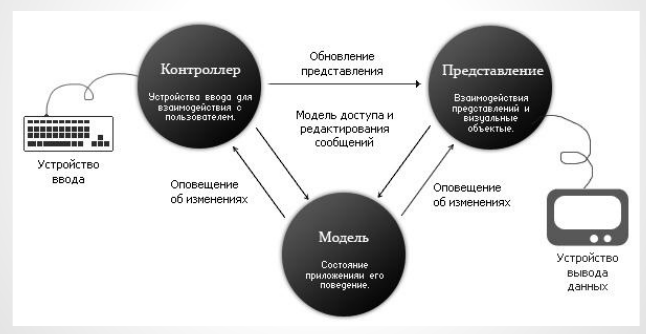
\includegraphics[width=0.9\textwidth]{mvc}
\caption{Архитектура веб-приложения}\label{web}
\end{figure}

За счет наличия исполняемой части, веб-приложения способны выполнять практически те же операции, что и обычные Windows-приложения, с тем лишь ограничением, что код исполняется на сервере, в качестве интерфейса системы выступает браузер, а в качестве среды, посредством которой происходит обмен данными, -- Интернет. К наиболее типичным операциям, выполняемым веб-приложениями, относятся:
\begin{enumerate}
\item прием данных от пользователя и сохранение их на сервере;
\item выполнение различных действий по запросу пользователя: извлечение данных из базы данных (БД), добавление, удаление, изменение данных в БД, проведение сложных вычислений;
\item аутентифицирование пользователя и отображение интерфейса системы, соответствующего данному пользователю;
\item отображение постоянно изменяющейся оперативной информации и т.д.
\end{enumerate}

Современные веб-приложения -- это порталы, предоставляющие услуги. Более четкую иерархию веб-приложений можно посмотреть на рисунке \ref{type_sites}
В настоящее время с точки зрения назначения различают три основных типа порталов:
\begin{enumerate}
\item Публичные, или горизонтальные, порталы (называемые иногда мегапорталами), такие как Rambler. Такие порталы нередко являются результатом развития поисковых систем. Предназначены они для самой широкой аудитории, что отражается на содержании предоставляемой ими информации и услуг. Как правило, эта информация носит общий характер, равно как и предоставляемые услуги (электронная почта, новостные рассылки и так далее).
\item  Вертикальные порталы. Этот вид порталов предназначен для специфических видов рынка. Вертикальные обслуживает аудиторию, пользующуюся услугами этого рынка или работающую на нем. Примерами таких порталов могут служить туристические агентства, предоставляющие услуги по бронированию мест в гостиницах, заказу и доставке билетов, доступу к картам и сведениям об автомобильных маршрутах. Или порталы типа business-to-business, позволяющие своим клиентам реализовывать совместные бизнес-операции (например, выбирать поставщиков и осуществлять закупку товаров, проводить аукционы).
\item Корпоративные порталы предназначены для сотрудников, клиентов и партнеров одного предприятия. Пользователи такого портала получают доступ к предназначенным им сервисам и приложениям в зависимости от их роли и персонального профиля[3].
\end{enumerate}

\begin{figure}[ht]
\center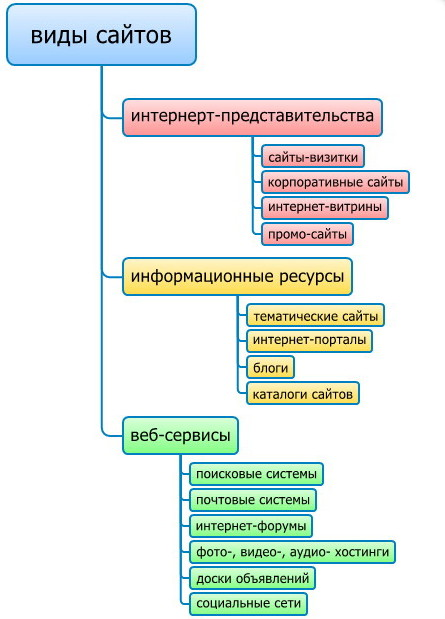
\includegraphics[width=0.5\textwidth]{type_sites}
\caption{Иерархия веб-приложений}\label{type_sites}
\end{figure}

Другие наиболее распространённые веб-приложения:
\begin{enumerate}
\item Региональные Интернет-порталы, универсальные по своему направлению, но ограниченные географией заинтересованных посетителей (e1.ru).
\item Поисковые системы -- это Интернет-порталы, которые предназначены для того, чтобы предоставить их посетителю возможность найти сайты, на которых встречаются заданные слова или целые фразы (yandex.ru, google.ru).
\item Каталог -- это коллекция ссылок на сайты. Зачем же нужны каталоги, если есть поиск? Очень часто мы не знаем точно, что нам нужно, и не можем это сформулировать парой слов (mail.ru).
\item Электронные доски объявлений  являются местом в интернете, где практически любой желающий может оставить информацию ознакомительного, пригласительного или рекламного характера.
\item Форумы -- это специальные сайты или разделы на сайтах, предназначенные для того, чтобы посетители, оставляя свои сообщения, обменивались мнениями, задавали вопросы в поисках ответов.
\item Чаты -- являются еще одним местом для общения в Интернет, только его назначение не обмен мнениями на какую-то тему, а просто времяпрепровождение.
\item Интернет-магазины и аукционы[3].
\end{enumerate}


\section {Серверная часть}

На стороне сервера веб-приложение выполняется специальным программным обеспечением (веб-сервером), который и принимает запросы клиентов, обрабатывает их, формирует ответ в виде страницы, описанной на языке HTML, и передает его клиенту.

В процессе обработки запроса пользователя веб-приложение компонует ответ на основе исполнения программного кода, работающего на стороне сервера, веб-формы, страницы HTML, другого содержимого, включая графические файлы. В результате, как уже было сказано, формируется HTML-страница, которая и отправляется клиенту. Получается, что результат работы веб-приложения идентичен результату запроса к традиционному веб-сайту, однако, в отличие от него, веб-приложение генерирует HTML-код в зависимости от запроса пользователя, а не просто передает его клиенту в том виде, в котором этот код хранится в файле на стороне сервера. То есть веб-приложение динамически формирует ответ с помощью исполняемого кода -- так называемой исполняемой части.

{\itshape PHP } -- скриптовый язык. В первую очередь PHP используется для создания скриптов, работающих на стороне сервера, для этого его, собственно, и придумали. PHP способен решать те же задачи, что и любые другие CGI-скрипты, в том числе обрабатывать данные html-форм, динамически генерировать html страницы и тому подобное. Но есть и другие области, где может использоваться PHP.
Вторая область – это создание скриптов, выполняющихся в командной строке. То есть с помощью PHP можно создавать такие скрипты, которые будут исполняться, вне зависимости от веб-сервера и браузера, на конкретной машине.
И последняя область – это создание GUI-приложений (графических интерфейсов), выполняющихся на стороне клиента\cite{php}.

{\itshape VBScript} -- язык создания сценариев VBScript разработан фирмой Microsoft, является подмножеством достаточно распространенного в среде программистов языка Visual Basic разработки прикладных программ Windows-приложений. Как и его родитель, язык VBScript достаточно прост и лёгок в изучении.
Преимуществом его применения для создания сценариев является возможность использования, с небольшими корректировками, ранее написанных процедур на языках Visual Basic и Visual Basic for Application.
Функциональные возможности сценариев, написанных на VBScript, ничем не отличаются от возможностей сценариев JavaScript: динамические создание документа или его частей, перехват и обработка событий и так далее.
VBScript используется для написания сценариев клиента (в этом случае браузер должен иметь встроенный интерпретатор этого языка), а также для написания сценариев на сервере (в этом случае сервер должен поддерживать язык VBScript).
Для создания сценариев клиента используется набор объектов, аналогичный набору JavaScript. Объекты клиента и сервера отличаются друг от друга, но существует общая часть (ядро) объектов, используемых при разработке как сценариев клиент, так и сценариев сервера\cite{VBS}.

{\itshape Perl} -- скриптовый язык. Наиболее широко Perl используется для разработки инструментов системного администрирования, однако в последнее время он получил огромную популярность в области разработки Интернет-приложений: CGI-сценариев, систем автоматической обработки электронной почты и поддержки узлов Web\cite{perl}.
Вот некоторые примеры задач, которые можно решать с помощью Perl:
\begin{enumerate}
\item проверка пользователей Windows NT на несоответствие их статуса и возможностей;
\item управление NT-сервисами из командной строки и дистанционно с локальной машины получение статистических данных на отдельной машине;
\item может работать и с протоколом FTP;
\item системная поддержка UNIX и Windows.
\end{enumerate}

\section {Клиентская часть}

Отображением результатов запросов, а также приемом данных от клиента и их передачей на сервер обычно занимается специальное приложение -- браузер. Как известно, одной из функций браузера является отображение данных, полученных из Интернета, в виде страницы, описанной на языке HTML, следовательно, результат, передаваемый сервером клиенту, должен быть представлен на этом языке.
Рассмотрим основные инструменты, с помощью которых можно создать любой веб-сайт.

{\itshape HTML } --  язык разметки гипертекста (Hypertext Markup Language)  -- это компьютерный язык, лежащий в основе World Wide Web (Всемирной Паутины). Благодаря языку HTML любой текст можно разметить, преобразовав его в гипертекст с последующей публикацией в веб.
Язык HTML имеет собственный набор символов, с помощью которых веб-браузеры отображают страницу. Эти символы, называемые дескрипторами, включают в себя элементы, необходимые для создания гиперссылок.
Одной из отличительных особенностей HTML-документов является то, что сам документ содержит только текст, а все остальные объекты встраиваются в документ в момент его отображения Браузером с помощью специальных тэгов и хранятся отдельно. При сохранении HTML-файла в месте размещения документа создается папка, в которую помещаются сопутствующие ему графические элементы оформления\cite{php}.

Веб-сайт должен быть не только функциональным, но и привлекательным. Для того чтобы приукрасить обычную HTML-страницу, наполненную текстом, понадобиться инструмент {\itshape Cascading Style Sheets } -- формальный язык описания внешнего вида документа, написанного с помощью языка разметки.  CSS используется создателями веб-страниц для задания цветов, шрифтов, расположения отдельных блоков и других аспектов представления внешнего вида этих веб-страниц. Основной целью разработки CSS являлось разделение описания логической структуры веб-страницы (которое производится с помощью HTML или других языков разметки) от описания внешнего вида этой веб-страницы (которое теперь производится с помощью формального языка CSS). Такое разделение может увеличить доступность документа, предоставить большую гибкость и возможность управления его представлением, а также уменьшить сложность и повторяемость в структурном содержимом. Кроме того, CSS позволяет представлять один и тот же документ в различных стилях или методах вывода\cite{php}.

Но язык разметки не обладает логикой, не умеет обрабатывать данные -- только отображать. Для того чтобы наделить клиентскую часть функционалом и создать интерактивный HTML-документ, используют язык программирования {\itshape JavaScript }. Это прототипно-ориентированный сценарный язык разработки встраиваемых приложений, выполняющихся как на стороне клиента, так и на стороне сервера\cite{php}.
Основные области применения JavaScript делятся на следующие категории:
\begin{enumerate}
\item динамическое создание документа с помощью сценария;
\item оперативная проверка достоверности заполняемых пользователем полей форм HTML до передачи их на сервер;
\item создание динамических HTML-страниц совместно с каскадными таблицами стилей и объектной моделью документа;
\item взаимодействие с пользователем при решении <<локальных>> задач, решаемых приложением JavaScript, встроенном в HTML-страницу.
\end{enumerate}

Частая перезагрузка страницы снижает производительность и удобство работы с веб-сайтом. Для того чтобы на каждый запрос сервер не выдавал новую страницу, а отсылал лишь те данные, которые нужны клиенту, в HTML из них прямо в браузере формирует движок Ajax.
{\itshape Ajax } расшифровывается как Asynchronous Javascript And XML и технологией в строгом смысле слова не является. Он определяет, какие запросы можно обработать <<на месте>>, а за какими необходимо обращаться на сервер. Асинхронность проявляется в том, что далеко не каждый клик пользователя доходит до сервера, причем обратное тоже справедливо -- далеко не каждая реакция сервера обусловлена запросом пользователя. Большую часть запросов формирует движок Ajax, причем его можно написать так, что он будет загружать информацию, предугадывая действия пользователя\cite{php}.
Где стоит использовать Ajax:
\begin{enumerate}
\item Формы. Если асинхронно передавать данные, страница не перезагружается, что заметное ускоряет работу.
\item Навигация в виде <<дерева>>. Такая навигация не является удобной и лучше использовать простую топологию, но если уж до этого дошло, лучше использовать Ajax.
\item Голосования. Пользователю будет приятней оставить свой голос за несколько секунд, чем за 30-40.
\item Фильтры. Часто на сайтах делают сортировку по дате, по имени. Ajax это будет значительно удобнее.
\end{enumerate}

 
{\itshape jQuery}-- библиотека JavaScript, фокусирующаяся на взаимодействии JavaScript и HTML. Библиотека jQuery помогает легко получать доступ к любому элементу DOM, обращаться к атрибутам и содержимому элементов DOM, манипулировать ими. Также библиотека jQuery предоставляет удобный API для работы с Ajax. jQuery обладает широким спектром возможностей, главными из которых являются визуальные эффекты, Ajax-дополнения и JavaScript-плагины\cite{php}.


\clearpage